\chapter{Approach}\label{chap:approach}

In the field of unsupervised instance detection and segmentation, CutLER~\cite{wang2023cut} gives a strong performance by exploiting a  object-centric prior by training on ImageNet~\cite{deng2009imagenet}, as most images contain a single
object in the center of the frame.  Due to its strong instance discrimination abilities, CutLER is the current state-of-the-art method for this task.

In this chapter, we are exploring the limitation of CutLER, looking deeper into the special cases where CutLER fails such as overlapping instances, complex backgrounds etc. We also analyze the change in performance when the model is trained without overlapping instances, as a main reason for CutLER's superior  performance is it's object-centric prior~\cite{engstler2023understanding}. Using the gathered information from the analysis, we introduce a hypothesis to refine Maskcut masks using CutLER outputs to train the model from scratch to obtain a better evaluation score across a variety of datasets.

\section{Limitations of CutLER}
Even though CutLER is the state-of-the-art model for unsupervised instance detection and segmentation, it still has several drawbacks. We go through some of them in this section.

\subsection{Overlapping instances}
Identifying instances using an unsupervised instance detection or segmentation method presents significant challenges, especially when instances are closely positioned or overlapping in an image. In such scenarios, the algorithm must discern subtle differences in texture, color, and shape without the benefit of labeled training data. Overlapping objects often blend together, making it difficult for the model to accurately segment and differentiate them as distinct entities. This lack of explicit supervision complicates the model's ability to learn and generalize the spatial relationships and boundaries between objects. Moreover, unsupervised methods typically rely on clustering and feature extraction techniques, which may not be robust enough to handle the complexities of overlapping instances, leading to errors in segmentation and misidentification. 

The problem is not exclusive to CutLER, but most of the existing methods~\cite{engstler2023understanding, cond1_support_2, Wang_2022_CVPR} also address this issue. Solving this problem requires, for instance, the learning of an instance-variant representation, which is a challenging task.

\subsection{Noisy pseudo-ground truths}
Noisy pseudo-ground truths generated by MaskCut can significantly hinder the performance of CutLER. These pseudo-ground truths often contain inaccuracies due to imperfect initial segmentation, which can arise from factors like complex backgrounds, occlusions, and variations in object appearance. Such noise can mislead the model, causing it to learn incorrect features and boundaries, ultimately degrading the quality of instance detection and segmentation. The presence of noisy masks can lead to overfitting on incorrect patterns or failure to generalize properly across different instances. To mitigate these issues, techniques like iterative refinement, robust loss functions, and the incorporation of consistency constraints have been proposed. Tang et al.~\cite{Tang_2018_CVPR} and Wang et al.~\cite{ziegler2022selfsupervisedlearningobjectparts} explore these approaches, highlighting the importance of addressing noise in pseudo-ground truths to enhance the robustness of unsupervised instance detection and segmentation methods.

In CutLER, a self-training loop is implemented to iteratively refine the pseudo ground truth masks. Even though it improves the performance of the model till 3 self training loops, it can further improved by making some changes in the mask filtration process, which will be explained in the next section.

\section{Impact of Overlapping Instances}
\label{section:analysis_ol_instancs}
When instances are closely positioned or overlapping in an image, it often makes the model difficult to accurately segment and differentiate them as distinct entities \cite{kara2022image}. But as CutLER mainly benefits from it's object-centric prior from training on Imagenet~\cite{engstler2023understanding}, we introduce a hypothesis that CutLER when trained with images without overlapping instances of Imagenet might perform better than training with all images.

For this, we make use of ground truth bounding box annotations provided by Imagenet and remove the images with an overlap(IoU) of \(\tau > \text{10\%}\text{ and }\tau > \text{25\%}\) are removed from the training set. The model's performance is compared with model trained using all image. For completeness, we also train a model using images with overlapping instances only.

Through this approach, we expect to observe an improvement by using less training data. But using this method in unsupervised fashion is rather challenging. Due to the grouping of nearby instances, the process of filtering images with overlapping instance is extremely challenging.

\section{Mask Refinement}
Generating initial pseudo-ground truth masks using a pre-trained model or some heuristic methods may contain errors or inaccuracies. Hence, iteratively refining the pseudo-ground truth masks(self- training) is essential for improving the performance of the model. Iterative refinement helps in progressively reducing this noise, leading to cleaner and more reliable labels~\cite{xie2020selftrainingnoisystudentimproves}. Popular refinement methods incorporate strategies like thresholding, where only high-confidence predictions are used for retraining, or use ensemble methods to combine predictions from multiple models for more reliable masks. CutLER also uses this method to filer the masks.

\subsection{Proposed mask refinement}
Inspired by our analysis in Section~\ref{section:analysis_ol_instancs}, which emphasizes quality over quantity, we introduce an improved approach for mask refinement. Noting that the current mask refinement method in CutLER tends to include noisy masks in its pseudo ground truths, we propose to enhance the process by removing ambiguous masks from the ground truth instead of retaining them. This adjustment aims to improve the overall quality and reliability of the pseudo ground truths, leading to better model performance.

Instead of adding masks from Maskcut with IoU < 0.5 to the pseudo-ground truth, we refine the CutLER predictions by removing masks that have IoU < 0.5. This approach effectively eliminates potentially noisy masks from the pseudo-ground truth, ensuring higher quality and more accurate mask predictions.

Even though the method might improve the precision, as we are limiting the range of exploration by removing more masks, we expect the recall to decrease by a small factor. However, our experiments indicate that this change is negligibly small. Detailed results and analysis can be found in the Experiments section.

%\begin{figure*}[h]
%	\centering
%	\begin{subfigure}[b]{0.47\textwidth}
%		\centering
%		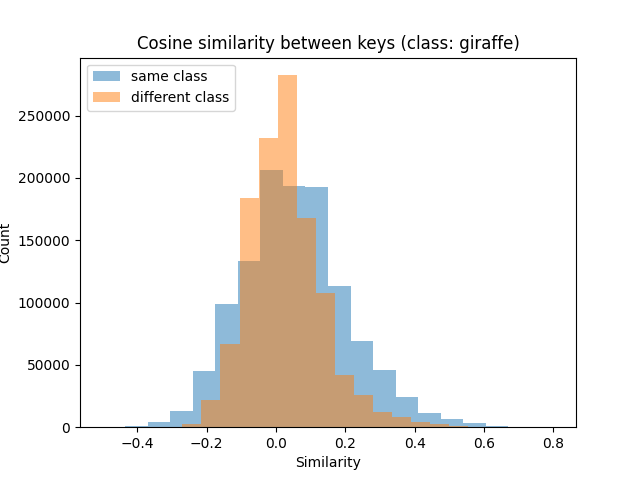
\includegraphics[width=\textwidth]{Images/same_vs_diff_class/plot_giraffe_cosine.png}
%		\caption{Cosine similarity}
%	\end{subfigure}
%	\quad
%	\begin{subfigure}[b]{0.47\textwidth}  
%		\centering 
%		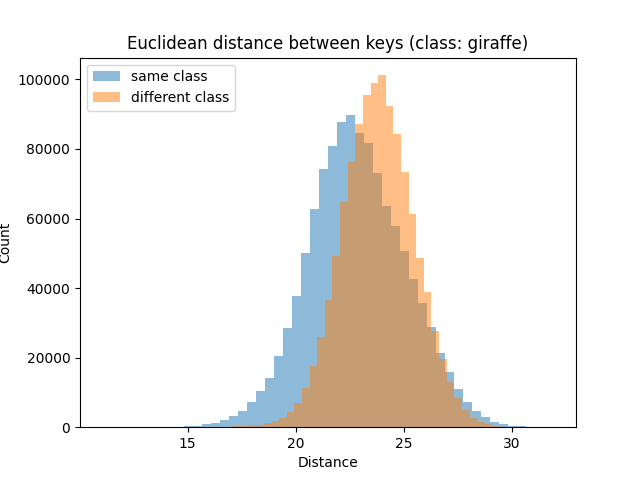
\includegraphics[width=\textwidth]{Images/same_vs_diff_class/plot_giraffe_euc.png}
%		\caption{Euclidean}
%	\end{subfigure}
%	\caption[\textbf{Comparison of keys of images of same and different classes}]{\textbf{Comparison of keys of images of same and different classes}. Shows the pattern of similarity scores and distance measure when comparing keys of same and different classes. Y axis shows number of images compared }
%	\label{fig:same_vs_diff}
%\end{figure*}